\documentclass[11pt,a4paper]{report}
\usepackage[utf8]{inputenc}
\usepackage[spanish]{babel}
\usepackage{amsmath}
\usepackage{amsfonts}
\usepackage{amssymb}
\usepackage{makeidx}
\usepackage{graphicx}
\usepackage{float}
\usepackage[left=1cm,top=1cm,right=1cm,bottom=1cm]{geometry} 
\begin{document}
	
	\begin{titlepage}
		
		\begin{center}
			\vspace*{-1in}
			\begin{figure}[t]
				\begin{flushleft}
					
\includegraphics[width=4cm]{LOGO_ITT_2005}
					
				\end{flushleft}
			\end{figure}
		
			
				\begin{huge}
					\vspace*{3cm}
					Pr\'actica 1.- Medici\'ones de Resistencias\\
					\vspace*{3cm}
				\end{huge}
			\begin{Large}
			
			Aguilar S\'anchez Jussef David \hspace{3cm}1810948\\
			Araujo Benito Noelia \hspace{4.4cm} 18210112\\
			Avila Dominguez Paulina \hspace{3.5cm} 18210113\\
			Carrillo Gonzalez Dominic Joselyn \hspace{1.8cm}18210114\\
			
			
			\vspace*{4cm}
		
				Profesor: Andrade Garc\'ia Juan Eduardo \\
			
			\vspace*{4cm}
			
				Tijuana Baja California a 18 de Febrero de 2019 \\
			\end{Large}
			
			\begin{figure}[b]
				\begin{flushright}
					
\includegraphics[width=0.4\linewidth]{BIOMEDICA_HEADING1-2048x672}
					
					\label{fig:biomedicaheading1-2048x672}
				\end{flushright}
				
			\end{figure}
			
		
		\end{center}
		
	\end{titlepage}


\newpage

	\begin{center}
	\begin{huge}
		Introducci\'on.\\
		\vspace*{1.5cm}
	\end{huge}
\end{center}

\begin{flushleft}
	
	El proposito de esta pr\'actica es aprender a realizar mediciones de resistencias por medio del mult\'imetro e interpretar el valor de las resistencias por medio de sus codigos de colores.\\
	\vspace*{0.5cm}
	
	Primeramente definiremos algunos conceptos.\\
	\vspace*{0.5cm}
	\begin{Large}
		Mult\'imetro.\\
	\end{Large}
	Es un instrumento de medida que ofrece la posibilidad de medir distintos parametros electricos y magnitudes en el mismo aparato. Las más comunes son las de voltímetro, amperímetro y óhmetro.\\
	\vspace*{0.5cm}
	Las diferentes funciones comunes en multimetros actuales son:\\
	Medición de resistencia\\
	Prueba de continuidad\\
	Medición de tensiones de CA y CC\\
	Medición de milivoltios de CA y CC\\
	Medición de corriente alterna y continua\\
	Medición de capacitancia (algunos modelos)\\
	Medición de frecuencia (algunos modelos)\\
	\vspace*{0.5cm}
	
	\begin{Large}
		Resistencia.\\
	\end{Large}
	
	Fuerza que rechaza o se opone a los electrones que se desplazan en algún material. La resistencia eléctrica se mide en Ohm. Una de las propiedades físicas de los materiales es su resistencia física a la electricidad. Según su resistencia se dividen en dos tipos:\\
	\vspace*{0.5cm}
	
	\textbf{Aislantes:} son materiales con gran resistencia eléctrica como lo son, por	 \vspace*{0.5cm} ejemplo, el plástico y la cerámica.\\ 	
	\vspace*{0.5cm}
	\textbf{Conductores:} permiten el libre flujo de los electrones debido a su baja resistencia eléctrica. Los metales, en general, son grandes conductores.\\
	\vspace*{0.5cm}
	La resistencia eléctrica varía dependiendo de otras características físicas del producto como:\\
	
	\textbf{El grosor:}: mientras más grueso el conductor menor es la resistencia.\\
	\textbf{La largura:} mientras más largo, mayor es la resistencia.\\
	\textbf{La conductividad:} mientras menor es la resistividad, mayor será la conductividad.\\
	\textbf{La temperatura:} a mayor temperatura, mayor será la resistencia.\\
	\vspace*{0.5cm}
	
	\begin{Large}
		C\'odigo de colores de las Resistencias.\\
		\vspace*{0.5cm}
	\end{Large}
	
	El c\'odigo de colores de las resistencias nos permiten conocer el valor en ohms que son capaces de soportar. En la mayoria de los casos las resistencias presentan 4 bandas de colores, cuando es asi se interpretan de la siguiente forma:\\
	\vspace*{0.5cm}
	
	\textbf{Bandas 1 y 2:}: representan los dos primeros valores de la resistencia.\\
	\textbf{Banda 3:} representa el factor multiplicador de la resistencia, es decir, los valores de las primeras dos resistencias se multiplicaran por el factor multiplicador de la tercer banda.\\
	\textbf{Banda 4:} representa el valor de la tolerancia de la resistencia, es decir, el valor obtenido de la resistencia puede varias + o - el valor encontrado en la cuarta banda respecto al valor obtenido en las 3 primeras bandas.\\
	\vspace*{0.5cm}
	
	Cuando la resistencia presenta una quinta banda, para obtener el valor de dicha resistencia se utiliza el procedimiento mencionado anteriormente pero la tercer banda tambien representara un numero, la cuarta banda representara al factor multiplicador y la quinta banda representara la tolerancia de la resistencia.\\
	
	
\end{flushleft}


\newpage
	\begin{center}
	\begin{Large}
		Desarrollo.\\
		\vspace{1.5cm}
	\end{Large}
\end{center}
\begin{flushleft}
	Lo primero que hicimos fue obtener los valores de cada una de las resitencias y compararlo con el  valor obtenido en la medici\'on, para ello nos apoyamos en una tabla del codigo de colores como la que se muestra a continuaci\'on:\\
	\vspace{0.5cm}
	\begin{figure}[H]
		\centering
		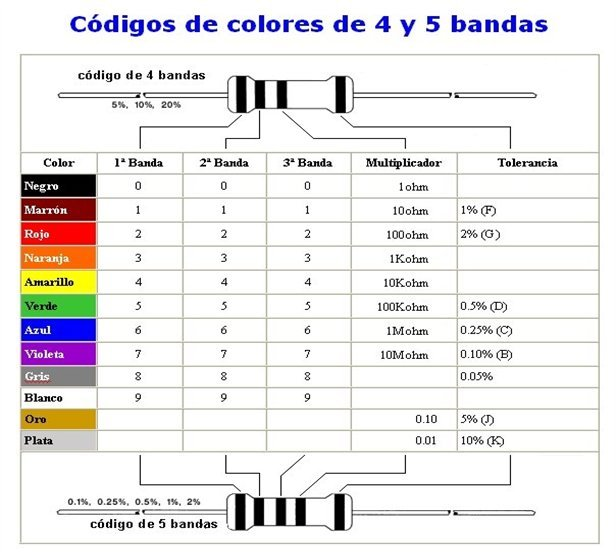
\includegraphics[width=0.4\linewidth]{bandas}
		\label{fig:bandas}
		\vspace{0.5cm}
	\end{figure}
	
	\begin{large}
		Resistencia 1.\\
	\end{large}
	
	La primer muestra de resistencia que medimos tenia un c\'odigo de colores de rojo, rojo, rojo, dorado como se muestra en la figura.\\
	\begin{figure}[H]
		\centering
		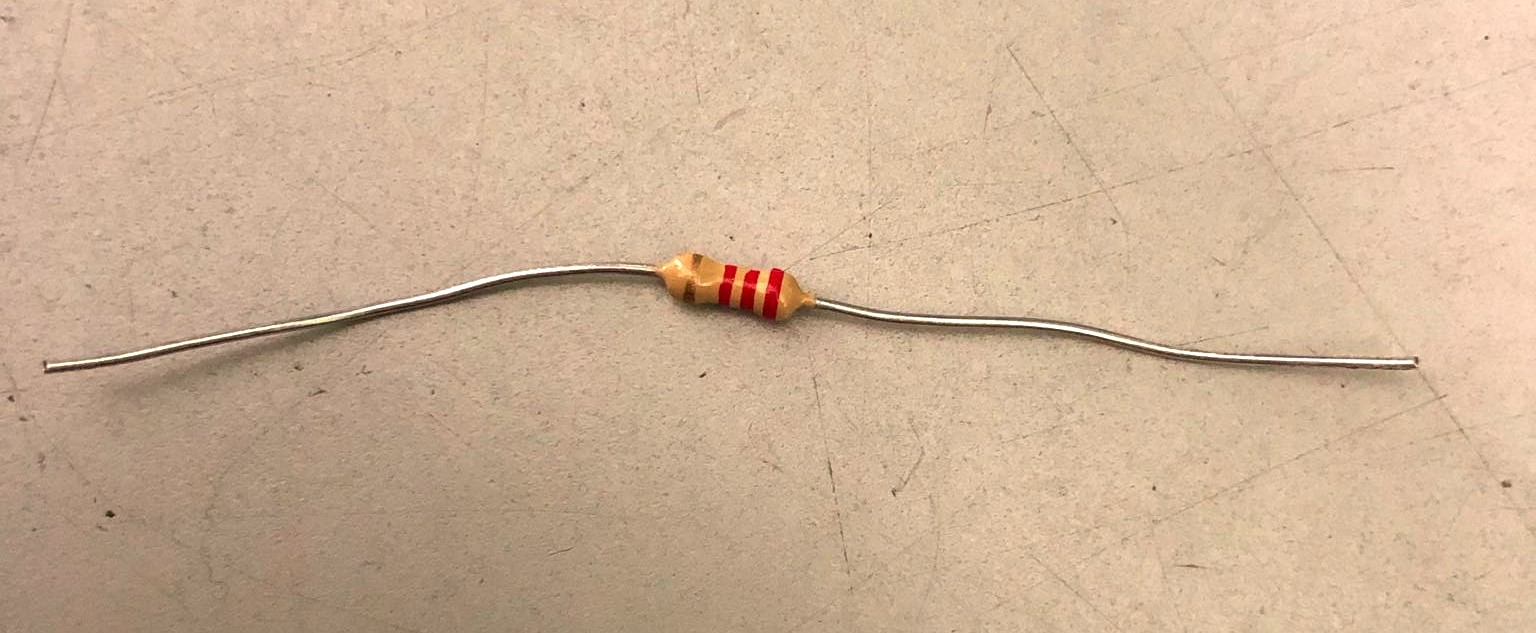
\includegraphics[width=0.4\linewidth]{resistencia1}
		\label{fig:resistencia1}
	\end{figure}
	
	Por lo tanto el valor de la resistencia es de 2200 ohms o 2.2 kohms.\\
	Y la medici\'on obtenida fue de 2.19 kohms como muestra la imagen.
	\begin{figure}[H]
		\centering
		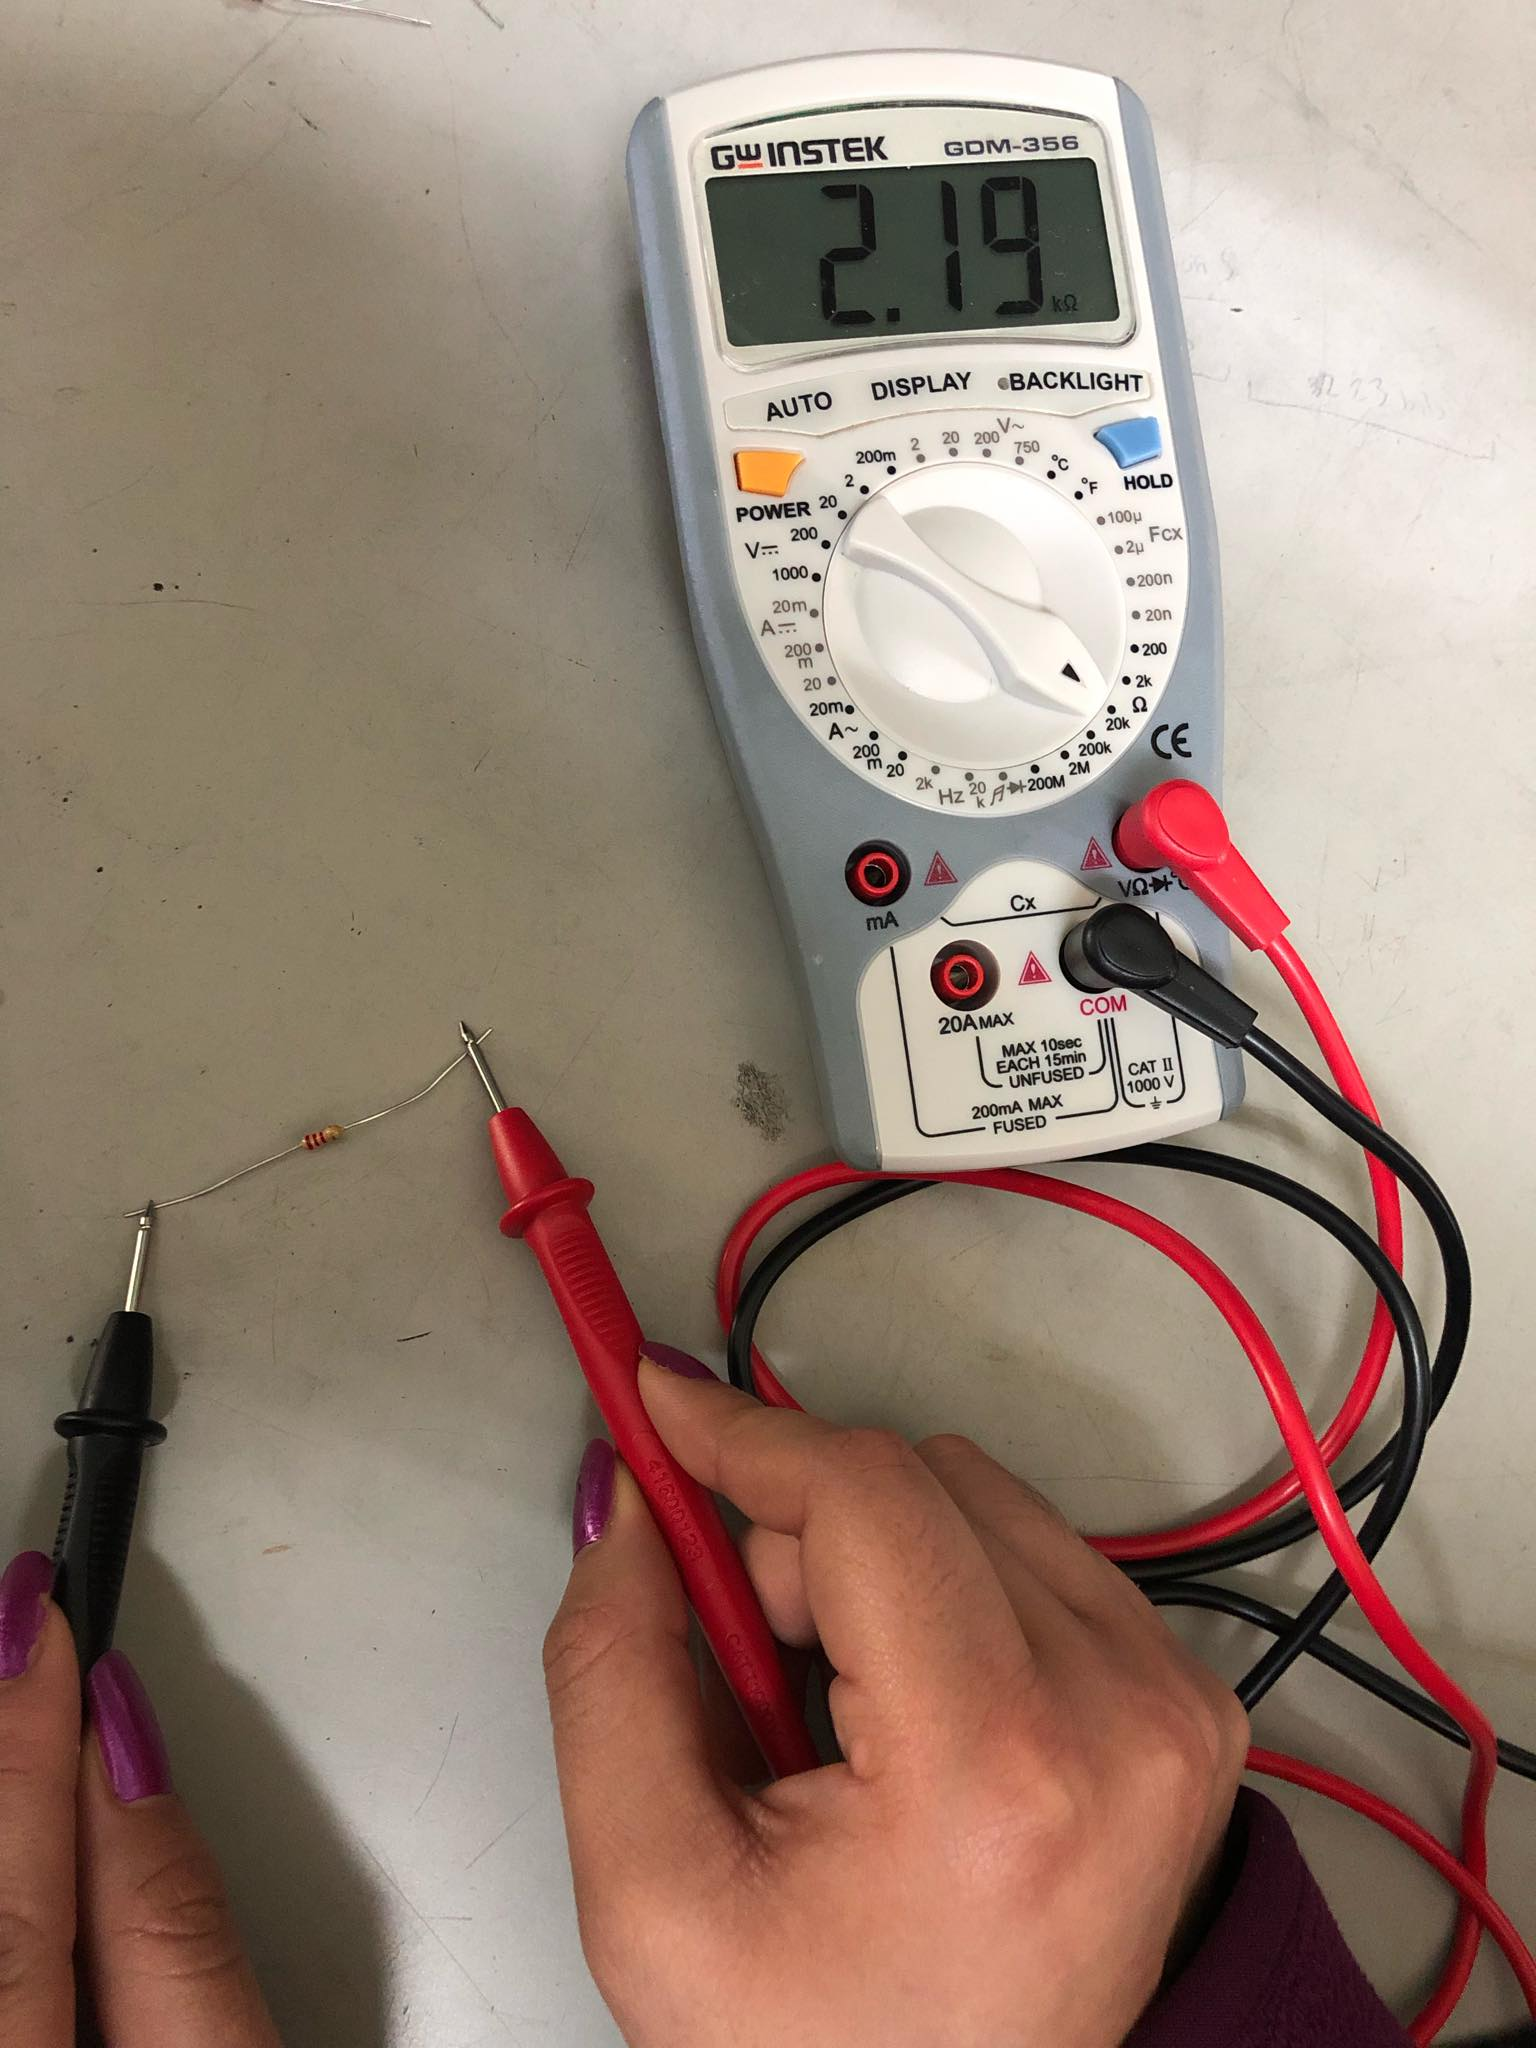
\includegraphics[width=0.3\linewidth]{medicion1}
		\label{fig:medicion1}
	\end{figure}
	\clearpage
	
	\begin{large}
		\vspace*{2cm}
		Resistencia 2.\\
	\end{large}
	La segunda resistencia que medimos tenia un c\'odigo de colores de rojo, negro, verde y dorado, como se muestra en la imagen.\\
	
	\begin{figure}[H]
		\centering
		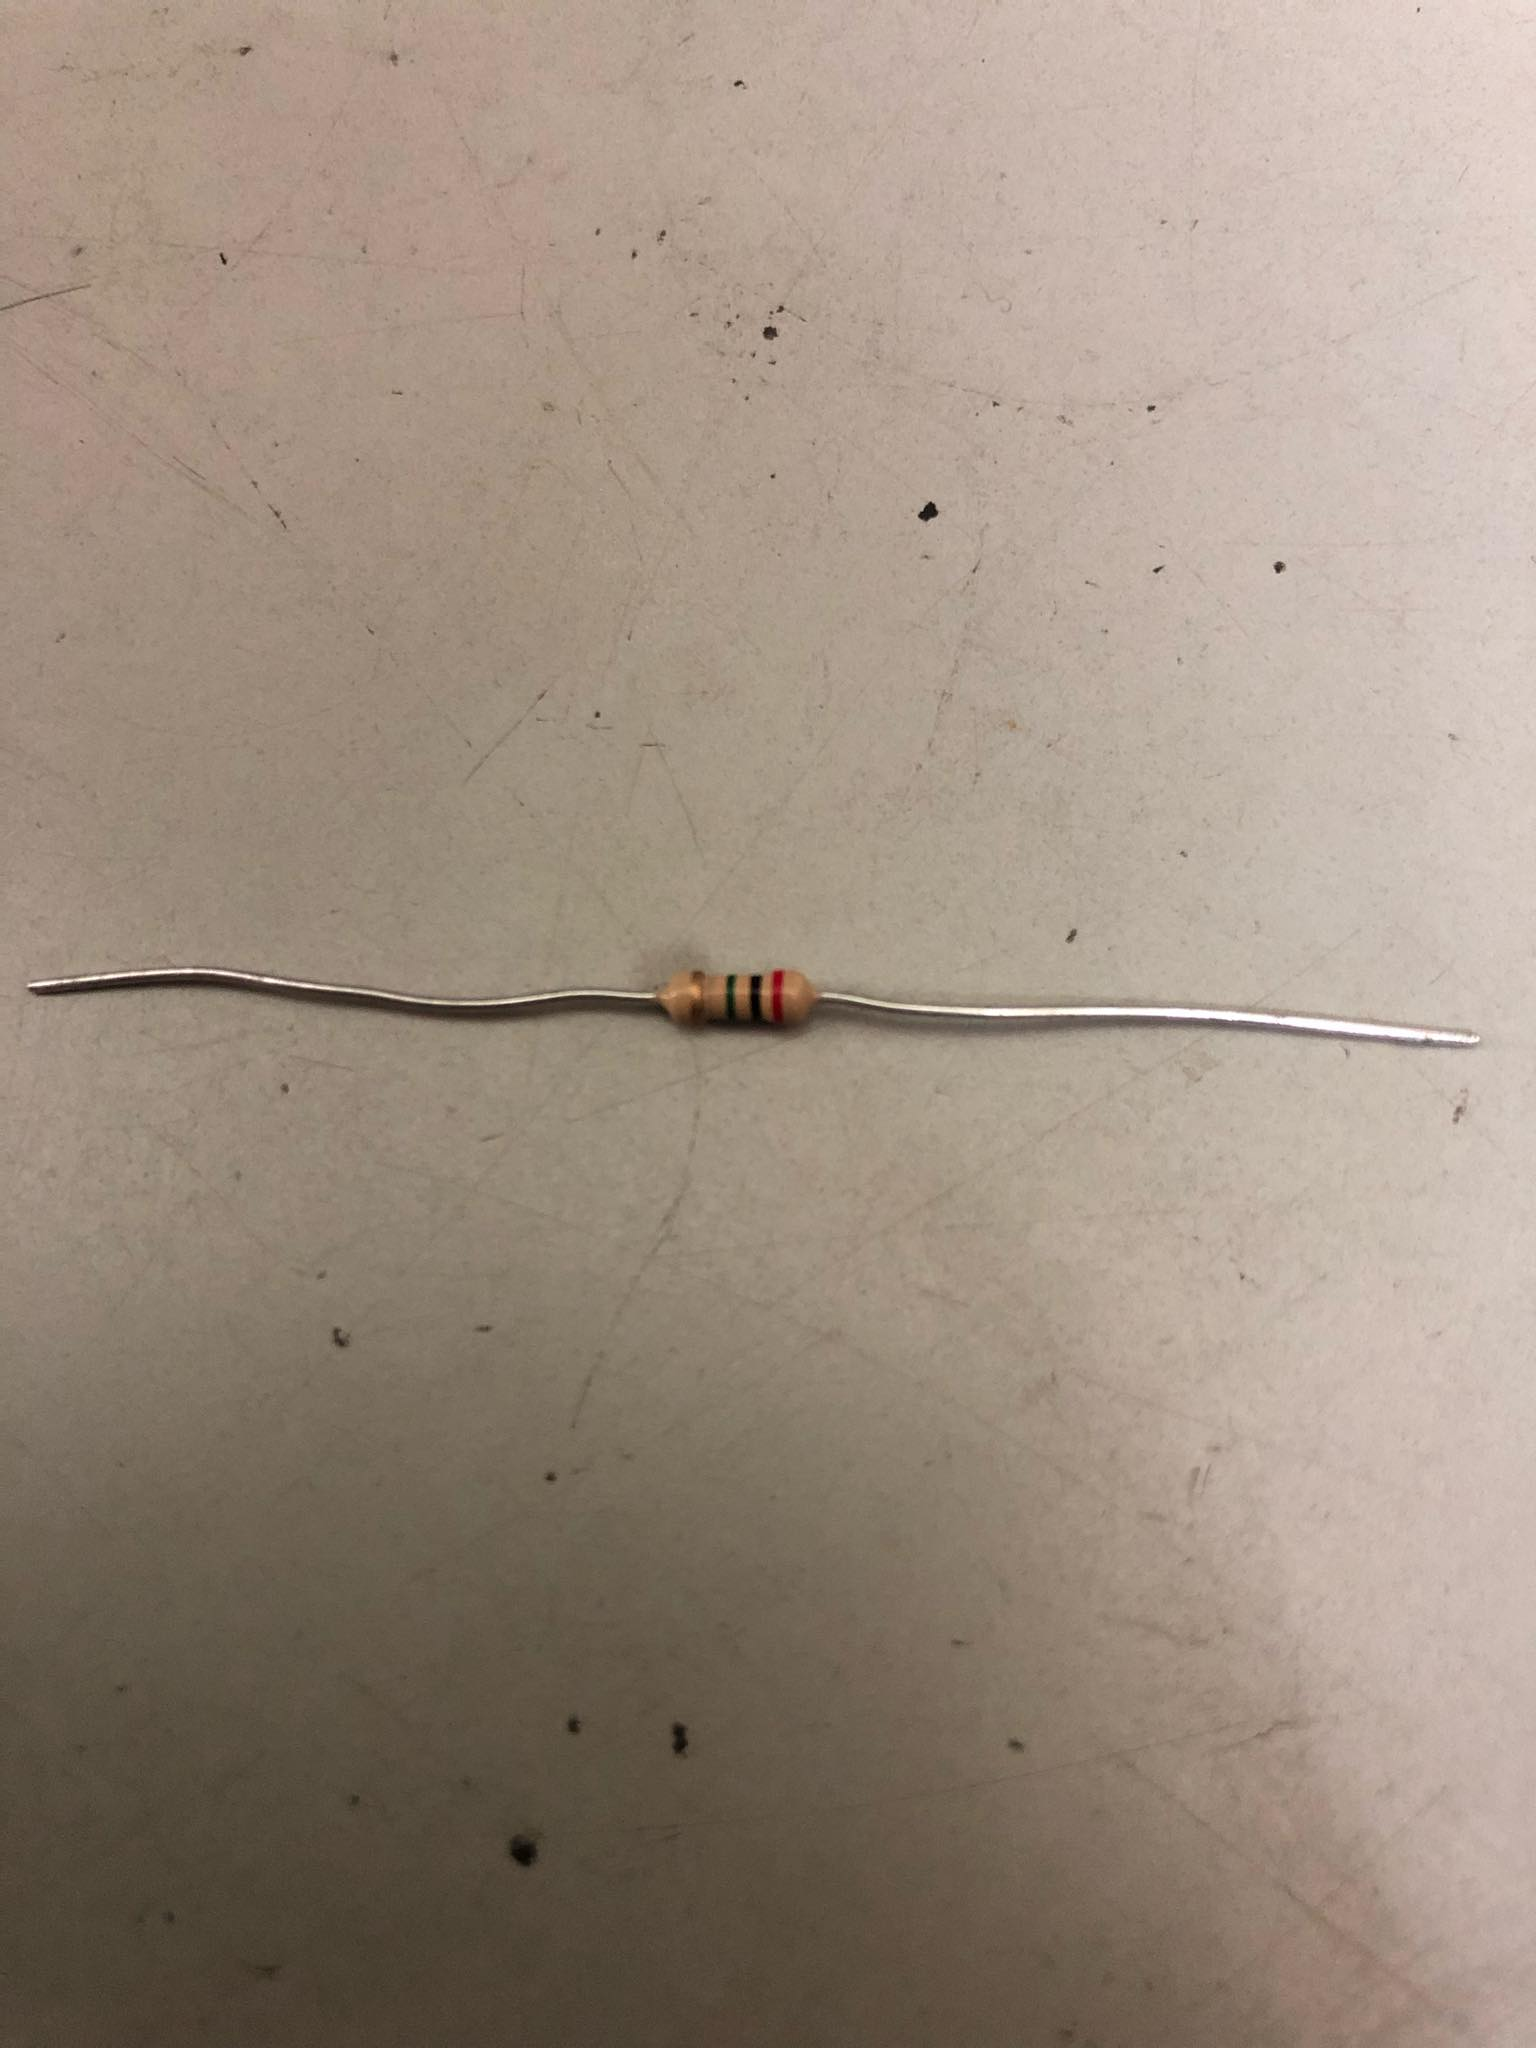
\includegraphics[width=0.4\linewidth]{resistencia2}
		\label{fig:resistencia2}
	\end{figure}
	Por lo tanto tenemos una resistencia con un valor de 2 MegaOhms.\\
	Y la medici\'on obtenida fue de 3 Megaohms, como muestra la imagen.\\
	\begin{figure}[H]
		\centering
		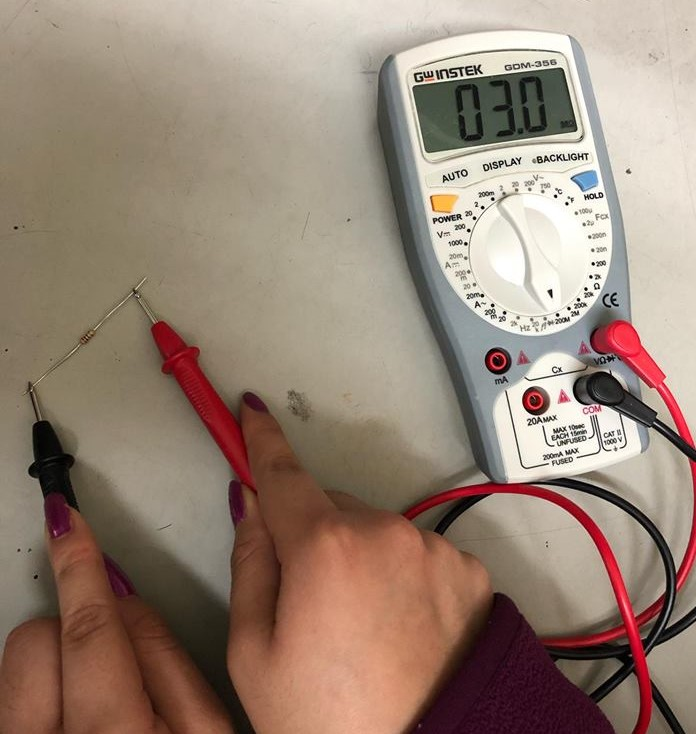
\includegraphics[width=0.3\linewidth]{medicion2}
		\label{fig:medicion2}
	\end{figure}
	
	\begin{large}
		\vspace*{2cm}
		Resistencia 3.\\
	\end{large}
	La tercera resistencia que medimos tenia un c\'odigo de colores de gris, rojo, caf\'e, y dorado, como se muestra en la imagen.\\
	
	\begin{figure}[H]
		\centering
		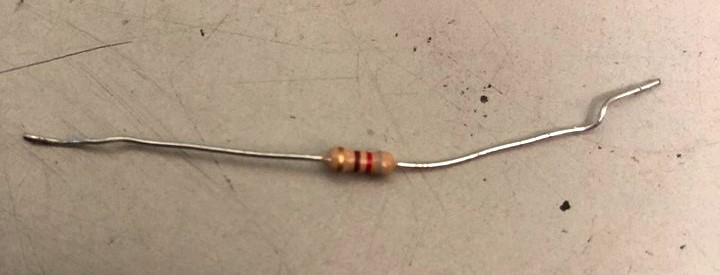
\includegraphics[width=0.4\linewidth]{resistencia3}
		\label{fig:resistencia3}
	\end{figure}
	\newpage
	\vspace*{2cm}
	Por lo tanto tenemos una resistencia con un valor de 821 Ohms \\
	Y la medici\'on obtenida fue de 810 Ohms, como muestra la imagen.\\
	\begin{figure}[H]
		\centering
		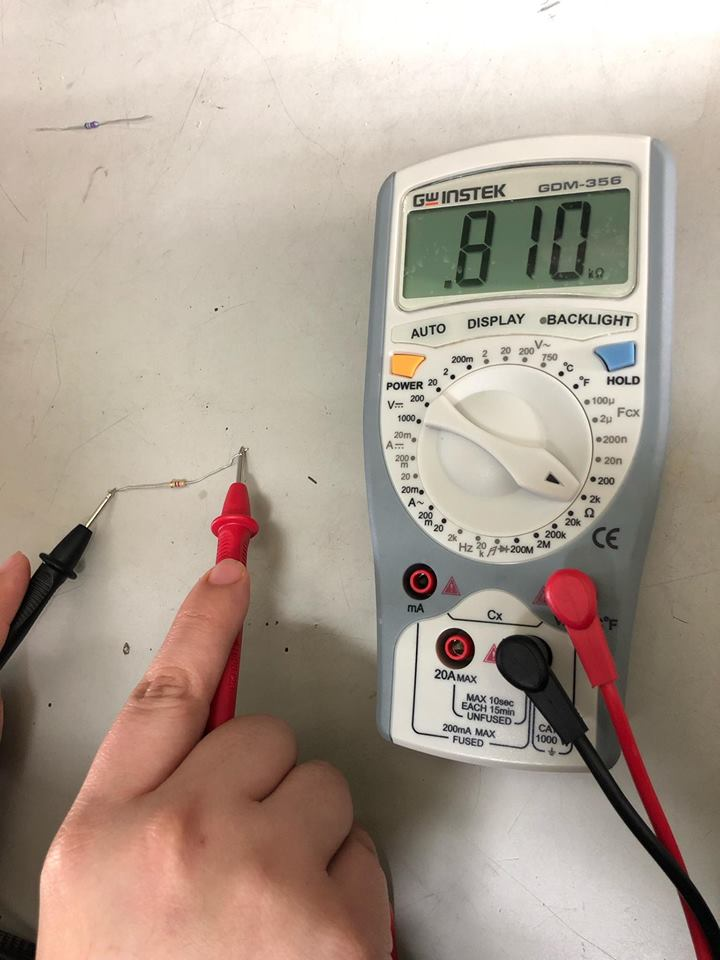
\includegraphics[width=0.3\linewidth]{medicion3}
		\label{fig:medicion3}
	\end{figure}
	
	\begin{large}
		\vspace*{2cm}
		Resistencia 4.\\
	\end{large}
	La cuarta resistencia que medimos ten\'ia un c\'odigo de colores verde, azul,amarillo y dorado, como se muestra en la imagen.\\
	
	\begin{figure}[H]
		\centering
		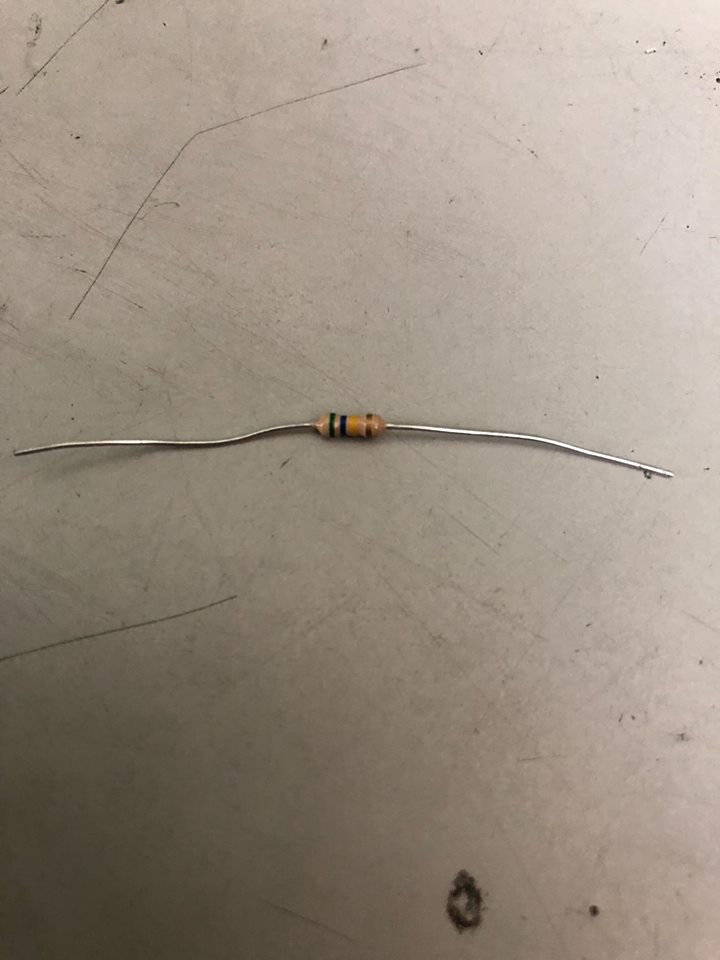
\includegraphics[width=0.4\linewidth]{resistencia4}
		\label{fig:resistencia4}
	\end{figure}
	Por lo tanto tenemos una resistencia con un valor de 564 Ohms \\
	Y la medici\'on obtenida fue de 581 Ohms, como muestra la imagen.\\
	\begin{figure}[H]
		\centering
		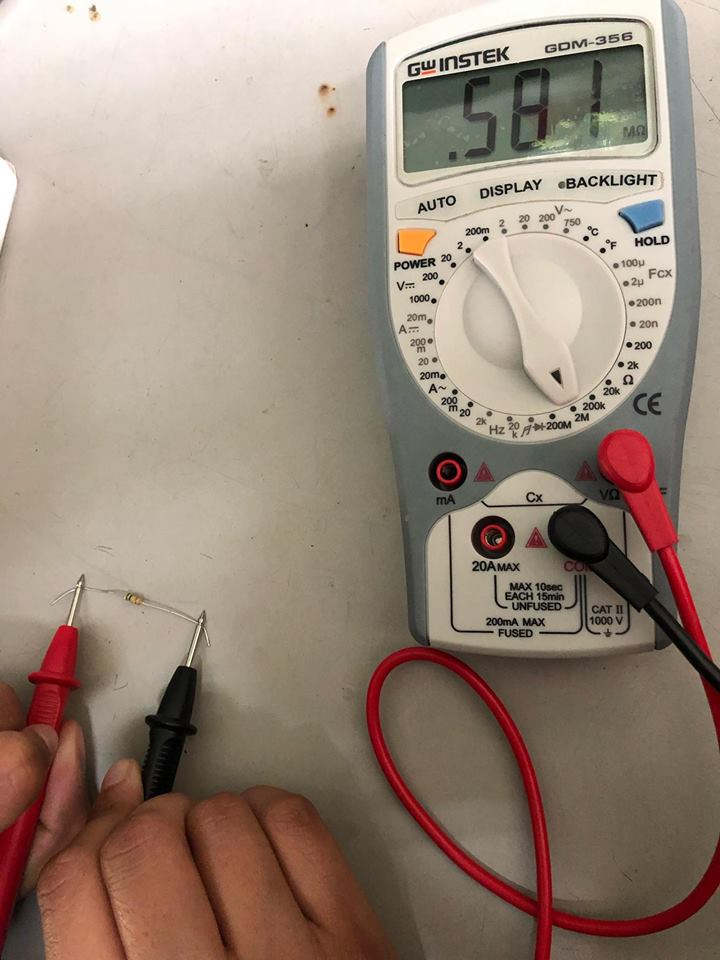
\includegraphics[width=0.3\linewidth]{medicion4}
		\label{fig:medicion4}
	\end{figure}
	
	\begin{large}
		\newpage
		\vspace*{2cm}
		Resistencia 5.\\
	\end{large}
	La quinta resistencia que medimos ten\'ia un c\'odigo de colores azul, amarillo,blanco, caf\'e,y marr\'on como se muestra en la imagen.
	
	\begin{figure}[H]
		\centering
		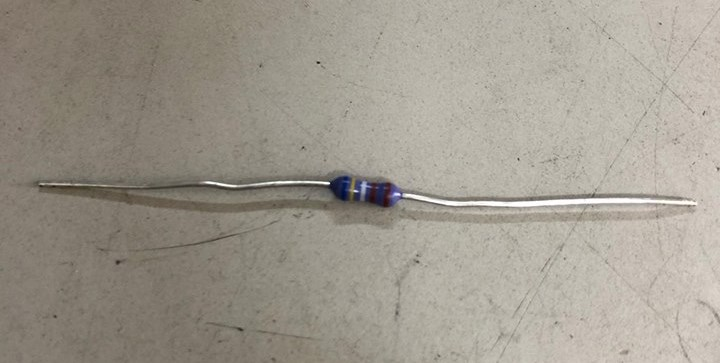
\includegraphics[width=0.4\linewidth]{resistencia5}
		\label{fig:resistencia5}
	\end{figure}
	Por lo tanto tenemos una resistencia con un valor de 6490 KiloOhms.\\
	Y la medici\'on obtenida fue de 6480 KiloOhms como se muestra en la imagen.\\
	\begin{figure}[H]
		\centering
		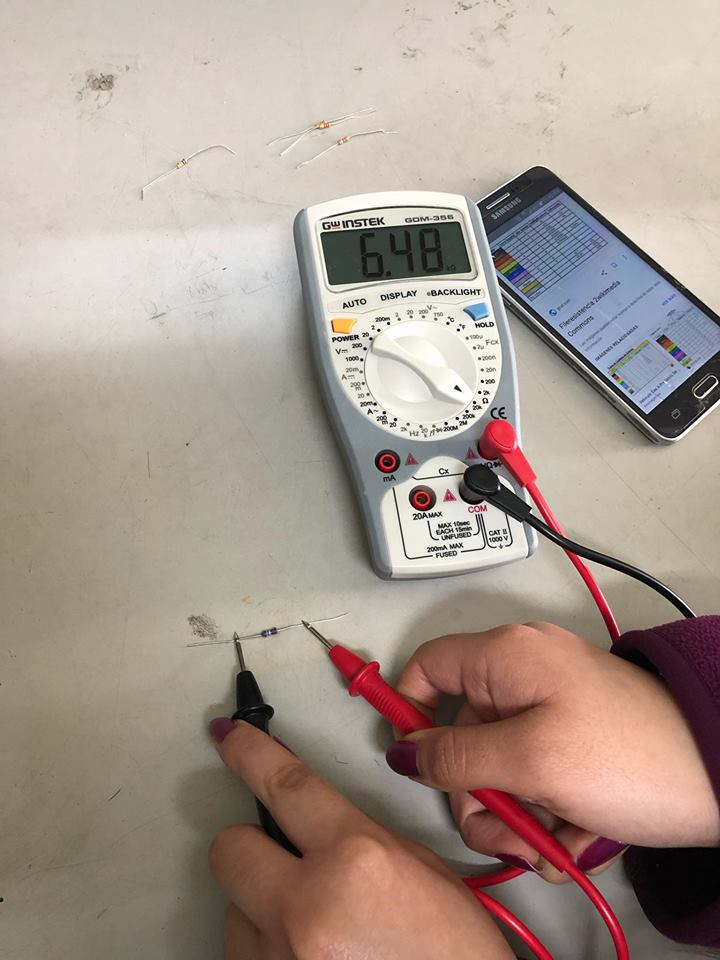
\includegraphics[width=0.3\linewidth]{medicion5}
		\label{fig:medicion5}
	\end{figure}
	
	
	
\end{flushleft}



\newpage

	\begin{center}
	\begin{Large}
		Conclusi\'on.\\
		\vspace{1.5cm}
	\end{Large}
\end{center}
\begin{flushleft}
	Al finalizar esta práctica se comprendió que los colores que contenían las 5 diferentes resistencias dadas por el docente tenían valores diferentes puesto que estos comprendían de diferentes colores, algunas de ellas comprendían de los mismos colores, pero variaban en la terminación dorada o plateada, pero esto no significaba que tenían el mismo valor.\\
	\vspace*{0.5cm}
	Con la ayuda de una tabla la cual contenía los valores de cada color presentado en la resistencia y algunos apuntes, el equipo se dio a la tarea de obtener los valores de las primeras líneas de colores y finalizando con una multiplicación de la penúltima línea del color designado en dicha resistencia. Después de obtener dicho valor se buscaba el valor exacto o cercano a este en el multímetro utilizado.\\
	\vspace*{0.5cm}
	Al finalizar la medición de cada una de las resistencias nos dimos cuenta que algunas de ellas sus valores no eran exactos ya fuese la medición o nuestro calculo, pero de ahí en fuera todo tenía el mismo valor calculado.
\end{flushleft}


\newpage

	\begin{center}
	\begin{huge}
		Bibliografia.\\
		\vspace*{1.5cm}
	\end{huge}
	\begin{flushleft}
		https://www.finaltest.com.mx/product-p/art-8.htm\\
		https://www.significados.com/resistencia-electrica/\\
		https://www.inventable.eu/2015/06/04/como-se-leen-los-colores-de-las-resistencias/\\
	\end{flushleft}
\end{center}
	
\end{document}